% TikZ 复刻。原图：assets/prism-placement.png
% 回退：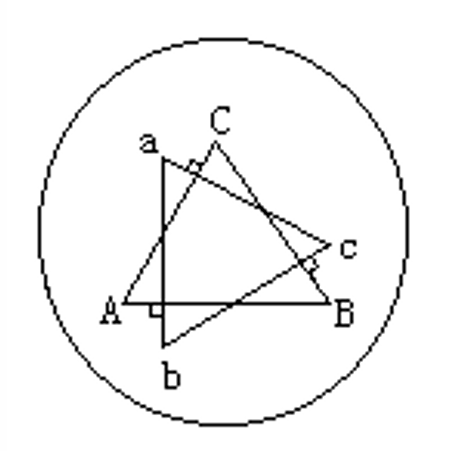
\includegraphics[width=0.72\linewidth]{assets/prism-placement.png}
% AB ⊥ 螺钉连线 a--b，AC ⊥ 螺钉连线 a--c。
\begin{tikzpicture}[font=\small]
  \def\R{2.20}
  \coordinate (O) at (0,0);
  \coordinate (Sa) at (210:\R);
  \coordinate (Sb) at (90:\R);
  \coordinate (Sc) at (330:\R);
  \draw[thick] (O) circle (\R);
  \draw[dashed] (Sa)--(Sb);
  \draw[dashed] (Sa)--(Sc);
  \filldraw[fill=white, thick] (Sa) circle (0.15);
  \filldraw[fill=white, thick] (Sb) circle (0.15);
  \filldraw[fill=white, thick] (Sc) circle (0.15);
  \node[below left] at (Sa) {$a$};
  \node[above] at (Sb) {$b$};
  \node[below right] at (Sc) {$c$};
  % constructed so AB ⊥ ab and AC ⊥ ac, vertex A toward screw a
  \coordinate (A) at (-1.15,-0.62);
  \coordinate (B) at (0.42,-1.48);
  \coordinate (C) at (-1.15,0.98);
  \draw[thick, fill=gray!15] (A)--(B)--(C)--cycle;
  \node[left] at (A) {$A$};
  \node[below right] at (B) {$B$};
  \node[above left] at (C) {$C$};
  \node[font=\scriptsize, rotate=70] at ($(B)!0.55!(C)$) {磨砂};
\end{tikzpicture}
